\chapter{La memoria}\index{memoria}
La memoria è un insieme di procedure mentali attive che consentono la conservazione dell’informazione per breve tempo (memoria a breve termine), la gestione e il recupero della conoscenza generale (memoria a lungo termine), suddiviso a sua volta in diversi sottosistemi specifici.

\section{Memoria a breve termine}\index{memoria!a breve termine}
La funzione della memoria a breve termine è quella di filtro rispetto alla miriade di stimoli che giungono al sistema. Essa trattiene per un breve periodo di tempo gli input sensoriali selezionati, insieme alle elaborazioni intermedie delle informazioni, finché non si trova una loro stabile destinazione. La memoria a breve termine è quindi la memoria di lavoro del sistema. A sua volta è suddivisa in due sottosistemi che gestiscono due tipi di informazioni. Il primo è visto come un \emph{loop articolatorio} in grado di registrare le informazioni e sovrascriverle in un paio di secondi. Il secondo invece memorizza le \emph{informazioni visive} e \emph{spaziali}. A questo sistema viene attribuita la creazione e la gestione delle immagini mentali e dei modelli mentali. I due sottosistemi lavorano in modo integrato fra loro grazie ad un meccanismo che le organizza e ne coordina l’attività, detto \emph{esecutivo centrale}.

La quantità di informazioni che la memoria a breve termine è in grado di gestire è limitata. George Miller\index{Miller, George}, nel suo famoso articolo \emph{The Magical Number Seven, Plus or Minus Two: Some Limits on Our Capacity for Processing Information} (1956), ha identificato la sua capacità massima, il cosiddetto \emph{memory span}\index{memory span}. Con questo termine si intende la più lunga lista di oggetti (per esempio numeri, lettere, parole, ecc) che una persona può ripetere nel corretto ordine immediatamente dopo l'acquisizione, nel 50\% delle prove. Miller osservò che il memory span di un giovane adulto è di circa 7 oggetti e che questo declina rapidamente al crescere del numero. Egli si accorse che è approssimativamente lo stesso con stimoli con una vasta differenza in merito al numero di informazioni, per esempio le cifre binarie hanno un bit ciascuna; le cifre decimali 3.32 bit ognuna. Lo psicologo concluse che il memory span non era limitato in termini di bit, ma piuttosto in termini di ``pezzi''.

\begin{figure}[hbt]
  \centering
  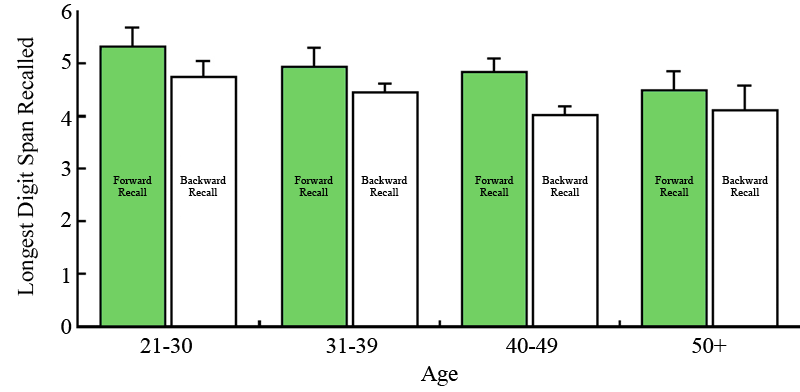
\includegraphics[width=\textwidth]{img/digit-span.png}
  \caption{Risultati tipici che possono essere ottenuti da un test di ripetizione numerica in avanti e indietro, raggruppati per età.}
  \label{fig:memory-span}
\end{figure}

Ci sono diversi fattori che influenzano il memory span, tutti studiati in esperimenti statistici. Alcuni di questi fattori, come le caratteristiche degli oggetti da memorizzare, il ritmo a cui essi sono presentati, le modalità con cui sono presentati, le distrazioni, sono estrinseci e riguardano l'esperimento in sé. Altri, come l'età (figura \ref{fig:memory-span}) e le condizioni patologiche, sono intrinseci delle persone e sono quelli che effettivamente stanno alla base del memory span.

\section{Memoria a lungo termine}
Si è stimato che la capacità di memorizzazione umana si aggiri attorno ai $10^9$ bit di informazione. La memoria a lungo termine opera da tramite fra la memoria a breve termine e la conoscenza del sistema. Questa può ricevere informazioni dalla memoria di lavoro per immagazzinarle nella conoscenza, oppure gestire e recuperare dalla conoscenza informazioni ben precise nel momento in cui servono.

\subsection{Memoria dichiarativa e procedurale}\index{memoria!dichiarativa}\index{memoria!procedurale}\index{conoscenza!esplicita}\index{conoscenza!tacita}
La memoria a lungo termine è generalmente divisa in due grosse categorie: la \emph{memoria dichiarativa} e la \emph{memoria procedurale}.

La memoria dichiarativa riguarda tutte le conoscenze esplicite (k-esplicita, esprimibile a parole) che si hanno sul mondo, mentre la memoria procedurale (k-tacita) non è verbalizzabile, e invece di essere una ``memoria di qualcosa'', è una memoria che riguarda il fare qualcosa, come andare in bicicletta, disegnare o fare l'amore. La memoria dichiarativa viene codificata nell'ippocampo, e poi depositata nelle aree associative, mentre la memoria procedurale è probabilmente codificata e immagazzinata nello striato e nel cervelletto: infatti, lesioni alle cortecce ippocampali ed entorinali possono compromettere selettivamente l'apprendimento di nuove nozioni, lasciando intatta la capacità di apprendere nuovi compiti motori.

La memoria dichiarativa a sua volta può essere suddivisa in altre sottocategorie: tra queste citiamo la \emph{memoria semantica}\index{memoria!semantica}, che riguarda conoscenze generali sul mondo esterno (ad esempio: tutto quello che una persona sa sui koala), e la \emph{memoria episodica}\index{memoria!episodica} (ipotizzata per la prima volta da Endel Tulving\index{Tulving, Endel} nel 1972), che, come suggerisce il nome, riguarda specifici episodi (ad esempio: la caduta del muro di Berlino), e le loro circostanze. Altri tipi di memoria sono quella \emph{autobiografica}\index{memoria!autobiografica}, che è un sottoinsieme della memoria episodica, e riguarda episodi della vita della persona, e la \emph{memoria prospettica}\index{memoria!prospettica}, che non riguarda, come le altre, eventi passati, ma eventi futuri (per esempio ``tra dieci giorni scadrà la bolletta'', oppure ``dopodomani alle dieci ho lezione'').

\section{Gestione della memoria}
\subsection{Immagazzinamento}
Le procedure di immagazzinamento, gestione e ricostruzione dei ricordi episodici sono le stesse che agiscono sulla memoria a lungo termine. Queste procedure memorizzano i dati forniti dalla memoria a breve termine e per questo motivo non lavorano su dati reali e oggettivi, ma dati che sono già stati elaborati dal sistema. Questa elaborazione può essere errata, quindi possono essere immagazzinati dati non corrispondenti con le percezioni di partenza. Due persone immerse nella stessa situazione ricorderanno il medesimo episodio in maniera differente in quanto lo hanno concettualizzato in modo diverso.

La conoscenza dipende quindi da come la memoria ha organizzato le informazioni in entrata, categorizzandole in modo arbitrario, secondo gli schemi interpretativi privilegiati dal sistema. I ricordi che vengono immagazzinati sotto forma di conoscenza tacita (memoria a lungo termine) veicolano il modo di procedere sia nell’ambiente esterno, sia interiormente. Questi ricordi possono essere attivati sia da strutture esplicite (azioni consce), sia da strutture tacite (sapori, odori, emozioni istintive).

\subsection{Gestione}
La capacità della memoria a lungo termine è finita, poiché basata su un sistema fisico finito, il cervello. Nonostante ciò la memoria sembra infinita: siamo sempre in grado di acquisire nuove informazioni e anche quello che non ricordiamo non è detto che sia perso per sempre, a volte le cose tornano in mente ed imparare cose già imparate in precedenza è più semplice.

La gestione riguarda il modo in cui i dati sono immagazzinati e strutturati e ricostruiti durante il ricordo. Le principali operazioni di gestione sono l’aggiornamento e la ristrutturazione dei sistemi di rappresentazione della conoscenza.

\subsection{Recupero}
Il recupero delle informazioni può avvenire dalla memoria k-tacita o da k-esplicita, ma comunque confluenti in un k-modello. Il recupero avviene attraverso strutture analoghe a quelle che hanno immagazzinato i ricordi. Questi schemi generali di conoscenza organizzano i dati singoli in insiemi significativi.

I \emph{frame}\index{frame interpretativi} sono le strutture espressive che la memoria usa per rendere leggibili i dati, fornendo l’interpretazione di ciò che è stato a suo tempo immagazzinato. I dati restano quindi stabili nel tempo, mentre ciò che si modifica sono gli schemi generali della conoscenza. Il passato non è accessibile se non attraverso le maschere interpretative dei frame, che vengono continuamente aggiornati. Così come percepiamo ciò che prevediamo di percepire, ricordiamo ciò che corrisponde alla nostra immagine del mondo oggi, e non agli schemi attivi quando l’evento è accaduto.

L’operazione di recupero quindi non è un semplice ripescaggio dell’informazione, piuttosto una complessa ricostruzione dei ricordi.

\subsection{Oblio}\index{oblio}
Le cause dell’oblio, ovvero della dimenticanza delle informazioni, va ricercata nelle disfunzioni delle procedure di immagazzinamento o di recupero. Per quanto riguarda l’immagazzinamento, esso ha a che fare con processi di decadimento o di interferenza. Il decadimento è dovuto principalmente al passare del tempo: ci si dimentica di un dato che non è stato più utilizzato. L’interferenza invece è causata dall’immagazzinamento di un numero rilevante di informazioni simili, che disturbano la nettezza del ricordo.

Quando invece è il recupero a non funzionare perfettamente, il soggetto è cosciente di avere in memoria quell’informazione, ma non riesce ad estrarla, come nel caso dell'anomia («ce l’ho sulla punta della lingua»).

Evidenze provenienti dalla clinica indicano che le informazioni che sembravano perse definitivamente sono invece recuperabili, se ci si impegna seriamente in quel compito. Analogamente, gli esperimenti sul trasferimento di conoscenza indicano che qualunque serie di dati, anche priva di senso, viene riappresa più facilmente rispetto ad una serie nuova, anche a distanza di mesi.

Si può concludere che l’oblio è dovuto essenzialmente a problemi di recupero o di attivazione delle informazioni, non ad una perdita delle stesse.

Un altro fenomeno interessante è quello dell’\emph{oblio infantile}\index{oblio!infantile}. È il fenomeno per cui gli adulti non riescono a ricordare le loro esperienze precoci, situate in un tempo precedente ai 4-5 anni. Esistono varie interpretazioni per questo fenomeno. Quella psicoanalitica si basa su meccanismi di soppressione dei ricordi dovuti ad ansia e sensi di colpa, quella neuropsicologica che sostiene che l’ippocampo (dove risiedono i ricordi) matura intorno ai 2-3 anni, causando la perdita di tutti i ricordi precedenti il suo pieno sviluppo. La spiegazione costruttivista, invece, si basa sul fatto che con la maturazione cambiano gli schemi di interazione con il mondo (frame mentali)\index{frame mentali}. I dati sono quindi presenti in memoria, ma non si è più in grado di recuperarli e ricostruirli in modo significativo mediante i nuovi schemi aggiornati.

\section{Modelli della memoria}
Sul finire degli anni '50, con l'emergere del cognitivismo il concetto di attenzione tornò al centro dell’interesse. Un esempio di modello che propone una selezione precoce dell’informazione da elaborare è stato proposto da D.E. Broadbent\footnote{Donald Eric Broadbent (Birmingham, 6 maggio 1926 – 10 aprile 1993), fu un influente psicologo sperimentale inglese. La sua carriera ha portato l'approccio psicologico pre Seconda Guerra Mondiale a quella che diventerà la psicologia cognitiva negli anni Sessanta.} tramite la \emph{teoria del filtro di Broadbent}\index{filtro di Broadbent}, secondo cui esisterebbe una fase iniziale di elaborazione dell’informazione durante la quale tutti gli stimoli vengono analizzati simultaneamente sulla base delle loro caratteristiche fisiche elementari e immagazzinati per un breve periodo.

In questa fase, quindi, non si ha alcuna selezione dell’informazione. A questo stadio di elaborazione, che Broadbent attribuisce al sistema sensoriale $S$, segue una fase di elaborazione più avanzata da attribuire al sistema percettivo $P$, il quale opera serialmente, elaborando cioè uno stimolo dopo l’altro. Un filtro, posto tra il sistema $S$ e il sistema $P$, seleziona gli stimoli che possono avere accesso ai livelli di elaborazione più sofisticati.

\begin{figure}[hbt]
  \centering
  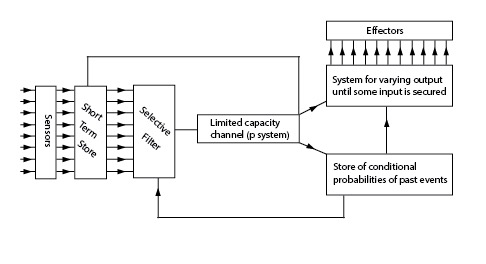
\includegraphics[width=\textwidth]{img/filtro-broadbent.jpg}
  \caption{Schema del filtro di Broadbent}
  \label{fig:broadbent}
\end{figure}

Broadbent asserì che i soggetti hanno la capacità di prestare attenzione ad una sola voce alla volta, evidenziando la relazione negativa, inversamente proporzionale, fra il grado di comprensione di due voci, nel senso che se aumenta la comprensione di una diminuisce la comprensione dell'altra (uso della tecnica dell'ascolto dicotico: stimolazione contemporanea di due canali sonori). Per seguire due processi gli individui devono alternare rapidamente l’attenzione dall’uno all’altro.

Annie Treisman modificò la teoria originale di Broadbent e formulò la \emph{teoria del filtro attenuato} (1964), detta anche della ``selezione tardiva'', secondo la quale il filtro attentivo si limita a ridurre, e non a cancellare, l’informazione disponibile nel canale non attentivo. Inoltre, in particolari condizioni, anche questa informazione ridotta è sufficiente ad attivare delle unità nel lessico mentale (una sorta di magazzino delle parole conosciute).

All’interno del lessico mentale esisterebbe uno stato di facilitazione di alcune unità che aumenterebbe la probabilità per certi significati (come ad esempio il proprio nome di battesimo) di essere attivati e quindi percepiti (effetto \emph{Cocktail party}). Negli esperimenti condotti da Treisman i soggetti erano sensibili all'informazione presentata all'orecchio cui si doveva prestare meno attenzione, soprattutto se la voce cui non dovevano prestare attenzione diceva il loro nome. Tale stato di facilitazione può infine essere modificato dalle istruzioni ricevute o dalle aspettative del soggetto.

\section{Working memory}\index{memoria di lavoro}
La memoria di lavoro (o working memory) è un modello che nasce nel tentativo di descrivere le dinamiche della memoria a breve termine. Grazie alla teoria dei \emph{livelli di elaborazione} (Craik e Lockhart, 1972), ed allo sviluppo delle tecniche di ricerca come il \emph{doppio compito} e l'\emph{interferenza selettiva}, nel 1974 viene proposto da Baddeley e Hitch un modello tripartito della working memory (poi perfezionato e integrato negli anni anche grazie alle evidenze neuropsicologiche), che prevede l'esistenza di un sistema attenzionale supervisore\index{esecutivo centrale} che controlla il flusso informativo, chiamato \emph{esecutivo centrale}, e di due sottocomponenti funzionali: il \emph{loop fonologico}\index{loop fonologico} ed il \emph{taccuino visuo-spaziale}\index{taccuino visuo-spaziale}. I sistemi gerarchicamente sottoposti all'esecutivo centrale sono magazzini a breve termine, dedicati alla ritenzione dell'informazione rispettivamente verbale e visuo-spaziale. Nel 2000, Baddeley ha aggiunto al suo modello una terza sottocomponente, chiamata \emph{episodic buffer}.

\begin{figure}[hbt]
  \centering
  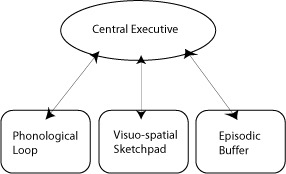
\includegraphics[width=0.5\textwidth]{img/working-memory.jpg}
  \caption{Rappresentazione gerarchica della working memory}
  \label{fig:working-memory}
\end{figure}

\subsection{Esecutivo Centrale}
L'esecutivo centrale è un sistema flessibile, responsabile del controllo e della regolazione dei processi cognitivi. Possiede le seguenti funzioni:

\begin{itemize}
  \item Coordinazione dei sistemi subordinati (slave systems);
  \item Coordinazione dell'esecuzione di compiti diversi nello stesso momento, e recupero di strategie;
  \item Attenzione selettiva ed inibizione.
\end{itemize}

Può essere concepito come un sistema supervisore, che controlla i processi cognitivi ed interviene quando essi non sono sufficienti.

\subsection{Loop fonologico}
Il loop fonologico si occupa interamente del trattamento dell'informazione fonetica e fonologica. È costituito da due sotto-componenti: un \emph{magazzino fonologico a breve termine}, cioè una memoria uditiva a rapido decadimento, ed un sistema di \emph{ripetizione articolatoria}, che evita il declino di una particolare traccia. Si assume che ogni stimolo verbale uditivo entri automaticamente nel magazzino fonologico.

Il magazzino fonologico può essere concepito come un ``orecchio interno'', grazie alle sue capacità di ritenere l'informazione sonora del discorso conservandone le proprietà temporali. Il sistema di ripetizione articolatoria invece, può essere concepito come una ``voce interna'', che grazie alla ripetizione subvocalica previene il decadimento delle tracce.

\subsection{Taccuino visuo-spaziale}
La memoria di lavoro visuo-spaziale (o ``visuo-spatial sketchpad''), intesa sia come capacità di mantenimento ed elaborazione di informazioni visuo-spaziali, che come capacità di generare immagini mentali, è stata studiata in maniera più approfondita a partire dagli anni '80 (Baddeley, 1986). In particolare, sono state messe in evidenza:

\begin{itemize}
  \item La distinzione tra materiale visivo e spaziale che corrisponde, come dimostrato da studi su pazienti e da studi sperimentali a due tipi di elaborazioni dissociabili (What \& Where).
  \item La distinzione tra elaborazione spaziale di tipo sequenziale e di tipo simultaneo.
  \item La distinzione tra elaborazione spaziale coordinata (relazioni spaziali in un sistema di riferimento geometrico euclideo), e l'elaborazione spaziale categorica (relazioni spaziali relative, come ``sopra'', ``a destra'', ecc) (Kosslyn, 1989).
\end{itemize}